\chapter{\uppercase{Design in the Presence of Uncertainty}}\label{OUUFramework}
\epigraph{``A product should be designed in such a way that makes its performance insensitive to variation in variables beyond the control of the designer''~\cite{Keane2005}}{---\textup{Genichi Taguchi}}

When a system is designed allowances must be made to accommodate likely variations that can disrupt the nominal performance, such as inaccuracies in modeling, uncertainties in manufacturing processes, operating environment and boundary conditions. 
When such variations or uncertainties are not accounted for in the design process, as in the case of a deterministic optimization practice, a degraded performance of the optimized design is inevitable.

\begin{figure}[h]
\centering
\begin{minipage}[b]{0.6\linewidth}
  \includegraphics[width=1.0\textwidth]{DeterVersusRobust.eps}
\end{minipage}
\caption{An illustration for the sensitivity of optimum designs to input variations.}
\label{fig:RobustDemo}
\end{figure}

In a heavily optimized design, the optimum solution tends to lie either at the extremum of the objective function or at the constraint boundary~\cite{Keane2005}. Thus, a deterministic optimum is a vulnerable solution with a greater likelihood of violating the design requirements: even small perturbations in the input can lead to a poor performance or failure of the design. To alleviate this, a factor of safety is traditionally incorporated into the constraints. For instance, in a structural design problem a stress constraint originally of the form $g(\d)=\frac{\sigma}{\sigma_{max}}-1\le 0$ is treated as $g(\d)=F_s\cdot\frac{\sigma}{\sigma_{max}}-1\le 0$, where $\d$ is the vector of design variables and \nom{$F_s$}{factor of safety} is the factor of safety. The factor of safety serves to move the optimum away from the constraint boundary by a considerable distance, thereby preventing the design from an imminent failure. However, the reality is that the designer assigning a factor of safety is seldom aware of the real effects of uncertainty and predominantly produces an over- or under-conservative design leading to weight penalty or vulnerable products, respectively. With the continuous evolution of radically new types of design, it is increasingly difficult for a designer to assign an adequate factor of safety~\cite{Keane2005}.

Due to these reasons, uncertainty quantification (UQ) has evolved as a field of interest, where the goal is to account for the effect of uncertainties through a modified optimization process known as \emph{optimization under uncertainty} (OUU).
OUU can be subdivided into two fields as \emph{robust design optimization} (RDO) and \emph{reliability based design optimization} (RBDO)~\cite{Arora2007,Agarwal2004,Padmanaban2003}. Though these two fields share many common attributes, they differ in their objectives: RDO techniques are used to produce a design that is more robust (less sensitive) to design parameter anomalies, whereas the goal of RBDO is to minimize the probability of failure of the system. This work focuses on methods to produce robust designs which involves finding an optimum that is less sensitive to input variability as opposed to a deterministic optimum that can exhibit a sharp change in the objective function value for minor perturbations in the inputs (see Figure~\ref{fig:RobustDemo}). 
Usually, a robust solution is obtained at the expense of an increased cost function~\cite{Keane2005} (also illustrated in Figure~\ref{fig:RobustDemo}). 

\paragraph{Stages in OUU:}There are three stages in design optimization under uncertainty~\cite{Keane2005}: 
\begin{enumerate}[(i)]
\item \emph{Identification, modeling and representation of uncertainties} to translate the available data into mathematical models that are either probabilistic or non-probabilistic in nature,
\item \emph{Propagation of  uncertainties} through computer models to quantify their impact on system performance,
\item \emph{Formulation and solution of an optimization problem} with appropriate objective and constraint functions ensuring that the optimum solution is robust against uncertainties.
\end{enumerate}
Brief overviews of these stages are provided in the remainder of this chapter. For an in-depth discussion on the subject, the reader is referred to works in the literature~\cite{Sandia2000,Sandia2006,Sandia2006b,Sandia2007,Sandia2008}.

\section{Uncertainty Modeling}
The modeling of uncertainties begins with the treatment of inputs as random variables. 
Uncertainties can be classified as \emph{aleatory} and \emph{epistemic} uncertainties~\cite{Sandia2000,Keane2005}. 
Aleatory uncertainties are the inherent randomness or variation in physical system, input parameters and variables,  or operating environment~\cite{Sandia2000}. For example, operating conditions are predominantly dissimilar to the ones used in design calculations and typically fluctuate around some mean value.
Epistemic uncertainties arise due to the lack of knowledge or information in any phase or activity of the modeling process. It is not an inherent property of the system and thus can be eliminated (or converted to aleatory form) when sufficient data becomes available. As an example, situations can arise where only the bounds or intervals of the uncertain random variables are known (e.g. manufacturing tolerances) whereas the underlying probability distribution or other statistical parameters within the interval are unknown (unlike aleatory random variables). 


\subsection{Probabilistic Modeling}

\begin{figure}[h]
\centering
\begin{minipage}[b]{0.49\linewidth}
\includegraphics[width=1.0\textwidth]{GaussHist.eps}
\end{minipage}
\begin{minipage}[b]{0.49\linewidth}
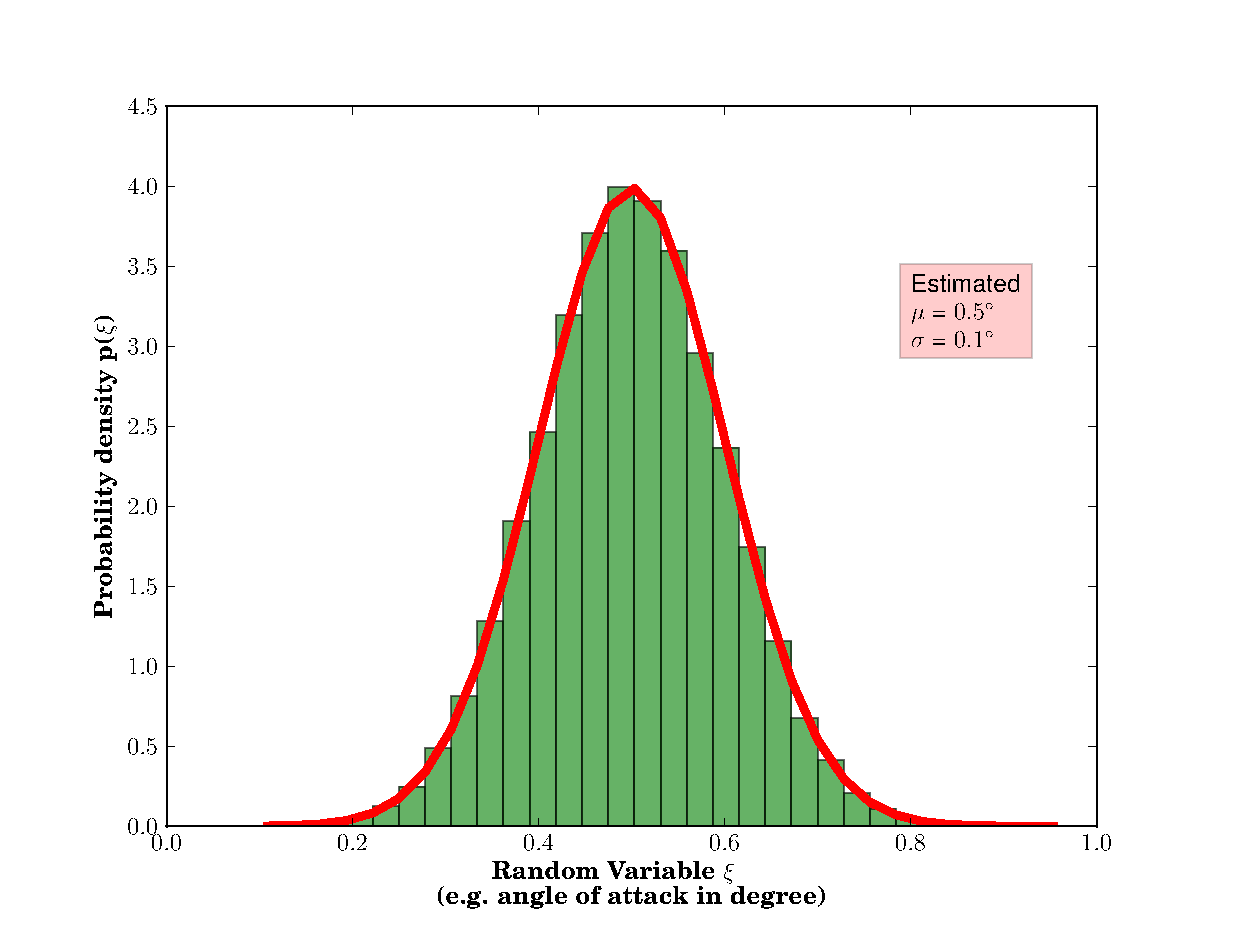
\includegraphics[width=1.0\textwidth]{GaussDemo.eps}
\end{minipage}
\caption[An illustration for the use of probabilistic uncertainty propagation methods.]{An illustration for the use of probabilistic methods. A histogram of the available angle of attack data (left) is shown with the fitted Gaussian probability density function (right) whose parameters ($\mu$ and \nom{$\sigma$}{standard deviation}) are estimated from the available data.}
\label{fig:GaussDemo}
\end{figure}


The use of probabilistic methods to model uncertainties is possible when sufficient data is available. When field data is available a probability density function can be fit to the available data.  Alternatively, a distribution function (Gaussian, log-normal, exponential, etc.) can be assumed and its parameters can be estimated from the available data. Figure~\ref{fig:GaussDemo} shows an example of fitting the available angle of attack information to a normal distribution function. The mean and standard deviation are estimated from the data and can be used to define the probability density function (PDF) of the random variable as $p(\xi)=\frac{1}{\sqrt{2\pi\sigma^2}}{e}^{-\frac{(\xi-\mu)^2}{2\sigma^2}}$ (Gaussian PDF). The angle of attack (and similarly any other variables) can now be treated as random variable in optimization formulations.

 Distributions should be assumed with caution when only limited data is available to the designer for assessment~\cite{Keane2005}. For example, a normal distribution  can not be assumed for Young's modulus, as a Gaussian distribution supports $[-\infty,+\infty]$ and a zero probability would mean a negative Young's modulus which is unrealistic. In reliability calculations, the probability of failure is estimated near the tail end of the distribution, which can be very erroneous if a wrong distribution structure is assumed. 

\subsection{Non-Probabilistic Modeling}

\begin{figure}
  \centering
  \includegraphics[width=0.60\textwidth]{rect.eps}    
  \caption{An illustration for bounds on input variables.}
  \label{fig:BoundsDemo}
\end{figure}

The use of probability theory to model the distribution of input uncertainties is questionable when not enough information is available. 
This naturally leads into non-probabilistic approaches such as possibility theory, interval analysis, convex modeling and evidence theory~\cite{Keane2005}.
The simplest non-probabilistic approach is perhaps the interval representation of input uncertainties. The input random variable is represented by the interval $[\eta^-,\eta^+]$ where $\eta^-$ and $\eta^+$ denote the lower and upper bounds on the input random variable, respectively. This scenario is illustrated with a two-variable example in Figure~\ref{fig:BoundsDemo}. The random process can take any value within the specified interval but the underlying probability distribution is unknown.
%and every value is equally likely, which is on the contrary to probabilistic approaches, where it is more likely for a value near the mean value to occur than the ones near the tail. 
The input bounds are processed into the analysis model to construct bounds on the output quantity of interest~\cite{Keane2005}. 


In summary,  probabilistic approaches are apt for modeling aleatory uncertainties featuring an abundance of data and non-probabilistic approaches are suitable for epistemic uncertainties suffering a data scarcity.

\section{Uncertainty Propagation}

In this section, approaches for the propagation of input uncertainties are discussed. The goal is to quantify the uncertainties and model the input--output relationship through numerical methods. The aleatory variables are denoted as \nom{$\z$}{aleatory variables/test candidate location} and realizations of aleatory variables from their probability distribution are represented as  \nom{$\bm{\alpha}$}{aleatory realizations}. The epistemic variables are denoted as \nom{$\n$}{epistemic variables} and their realizations within the specified bounds are denoted as \nom{$\b$}{epistemic realizations}.

\subsection{Propagation of Aleatory Uncertainties}\label{sampling}
Sufficient input data is generally available for the analysis of aleatory uncertainties. Thus, probabilistic methods which mandate multitude of realizations are commonly used for computing the statistics based on the input probability distribution. 
In other words, the distribution type of the input random variables (e.g. $\a \sim {\N}(\bar{\z},\bm{\sigma}_{\z}^2)$) are known, whereas the functional dependence $f(\z)$ on these random variables is not known, and are modeled using numerical simulations. 
\paragraph{Monte Carlo Simulation:}The simplest approach to achieve  uncertainty propagation is the Monte Carlo simulation (MCS). %, due to the presence of input statistical information 
When information such as the input mean, standard deviation and PDF of design variables and other parameters (collectively known as inputs) are available, the statistics of the output function can be computed using MCS. In this method, numerous samples (realizations) $\a^{(j)}$ are generated from the distribution $p(\z)$ of the input random variables and the response function or simulation code is evaluated. This leads to the following estimates for the mean:
\beq
\bar{f}=\mu_f=\dfrac{1}{\widetilde{N}}\sum_{j=1}^{\widetilde{N}}f(\a^{(j)}),
\label{Meanestimate}
\eeq
and variance of the output quantity:
\beq
\sigma^2_{f}=\var_f=\dfrac{1}{\widetilde{N}}\sum_{j=1}^{\widetilde{N}}(f(\a^{(j)})-\bar{f})^2,
\label{Varestimate}
\eeq
where \nom{$\widetilde{N}$}{number of Monte Carlo samples} is the number of Monte Carlo samples.
MCS can be used on any output function $f(\z)$ and is hence non-intrusive in nature.

\begin{figure}[h]
  \centering
  \begin{minipage}[b]{0.48\linewidth}
    \includegraphics[width=1.0\textwidth]{InputDistro.eps}\subcaption{Set of input variables with distributions}
  \end{minipage}
  \begin{minipage}[b]{0.48\linewidth}
    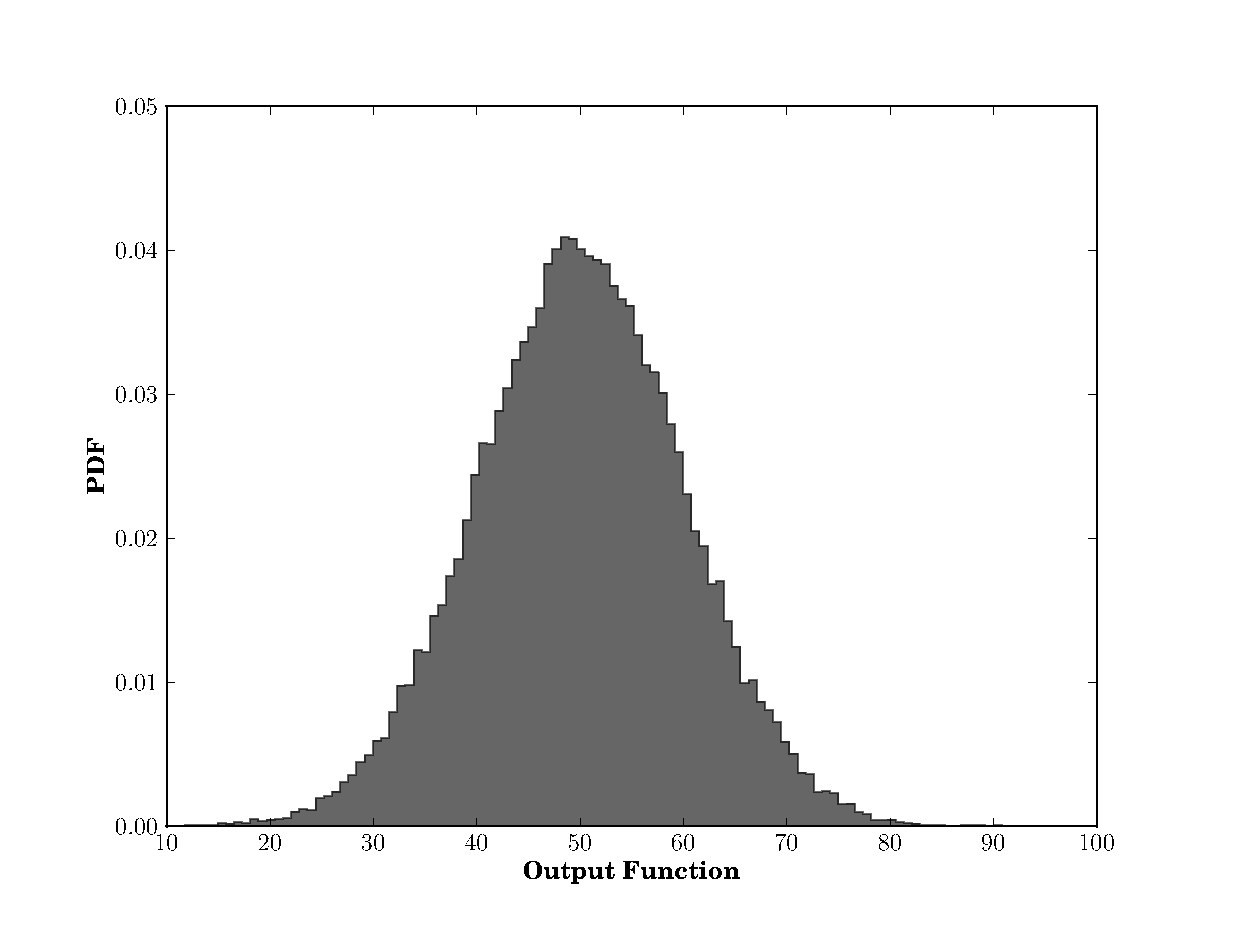
\includegraphics[width=1.0\textwidth]{outputdist.eps}\subcaption{Distribution of the output function}
  \end{minipage}
  \caption{An illustration for modeling the input-output relationship of uncertainties.}
  \label{fig:UQdemo}
\end{figure}

\paragraph{Inexpensive Monte Carlo Simulation:}It is known that repeated evaluations of the exact function, $f(\z)$, is prohibitively  expensive or impractical most of the times. To overcome this problem, surrogate models can be built and inexpensively probed to yield approximated output function values $\widehat{f}(\z)$ for the calculation of approximate means and variances. 
The required number of function values (training points) for building an accurate surrogate is usually way less than the number required for statistically converged Monte Carlo simulation. In this work, the domain over which the surrogate model is built is taken to be \emph{three standard deviations} in all aleatory input dimensions from the specified mean value \ie~ the surrogate domain is:  $[\bm{\bar{\xi}}\pm3\cdot\bm{\sigma_{\xi}}]$. %\bm{\alpha}^{(i)}\in
This implies that for normally distributed input variables more than $99$ \% of all samples (aleatory realizations) fall within the surrogate domain and the less accurate extrapolation capabilities of the surrogate model only need to be employed for a small fraction of the samples. A larger domain can be specified for the surrogate (e.g. $6\sigma$ from mean) to account for even remote possibilities, but is not used in this work (recommended for reliability calculations).
In this work, polynomial chaos and kriging surrogate models described in chapter~\ref{surrogatemodels} and trained using the dynamic framework described in chapter~\ref{TPSFramework} are employed for aleatory uncertainty propagation. Both surrogate models have the capability to incorporate higher-order derivative information (gradients and Hessian), however, the surrogates are built using function values only to reduce the complexity in presenting the results. %, but one could easily incorporate higher-order derivative information if desired. Figure~\ref{fig:UQdemo} provides an example of modeling the effect of input uncertainties on the output quantity of interest. 

%\subsubsection{Obtaining Derivative of Mean and Variance}

\subsection{Propagation of Epistemic Uncertainties}\label{probepis}

Epistemic uncertainties  represent the lack of knowledge about the appropriate value to use~\cite{Sandia2006b}. 
For instance, manufacturers typically provide intervals in terms of tolerances (e.g. $\pm~0.5~mm$ for length of a bolt), but the exact values are not known or cannot be guaranteed whatsoever. 
Here, the goal is  to have bounds on the output quantity of interest or to determine worst case scenarios (e.g. maximum possible constraint violation, least possible lift), in order to minimize the sensitivity or variation of the design with respect to these uncertainties.
In a situation where only the input interval $I(\n)=[\n^-,\n^+]=[\bar{\n}-\e,\bar{\n}+\e]$ is known, the above assessment can be accomplished in most straightforward manner by either one of the two methods discussed below.

\paragraph{Sampling:}\label{samp}

An extensively sampling of the interval $I(\n)$ can be done and the analysis of the resulting outputs $f(\n)$ is carried out to determine the extreme values (worst and best cases). However, the computational burden can be prohibitive in the case of high-fidelity physics-based simulations and for 
higher-dimensional spaces. As a remedy, a surrogate model over the domain $I(\n)$ can be constructed (similar to aleatory uncertainties), which can then be sampled using inexpensive Monte Carlo simulations (IMCS). 
However, with increasing number of variables, building an accurate surrogate model requires thousands of simulation outputs  (referred to as the curse of dimensionality) and quickly becomes prohibitively expensive as well.


\paragraph{Bound-Constrained Optimization:}\label{bco}
A  bound- or box-constrained optimization (BCO)~\cite{Lockwood2011,Lockwood2012a,Lockwood2011a} can be employed to find the worst and best behavior of the constraint/objective function within the specified interval $I(\n)$.  
A gradient-based BCO scales mildly with the number of input variables, making it computationally more attractive than MCS for quantifying the effect of epistemic uncertainties, particularly for larger problems. 
In BCO, the problem of finding the extreme value of the function, \nom{$f^*$}{extremum of the function within the  bounds}, (and the constraints, \nom{$g_i^*$}{extremum of the constraints within the bounds}) within the interval $I(\n)$ can be cast as follows:
\beq \label{eq:subopt}
\begin{aligned}
& \underset{\b}{\text{minimize/maximize}}
& & f=f(\n), \\
& \text{subject to}
& &  \b \in I(\n)=[\bar{\n}-\e,\bar{\n}+\e].\\
%& & & g^r=g(\mus,\q,\z,\n) - k \sigma_g^*  \le 0.\\
%& \text{bounds}
%& & \d^\text{L} \le \d \le \d^\text{U}.
\end{aligned}
\eeq
In most cases the extremum occurs at either the upper or lower bound of the interval due to the quasi-linearity of the typically small space described by $I(\n)$. 
Thus, BCO typically takes only about five to ten simulation output and gradient evaluations to reach $f^*$ and is used throughout this work to propagate epistemic uncertainties.
An L-BFGS~\cite{MyBFGS1,MyBFGS2} algorithm which utilizes function and gradient information is used to solve the BCO problem given by Eq.~\eqref{eq:subopt}.
\subsection{Propagation of Mixed Uncertainties}

Table~\ref{tab:compreq} summarizes the four typical methods that can be employed for the propagation of mixed epistemic and aleatory uncertainties along with their corresponding approximate simulation requirements. 
The computational requirements can be interpreted assuming an approximate range of values for: $(i)$ the number of Monte Carlo sample points ($\widetilde{N}=10^5 - 10^8$),  
$(ii)$ the number of surrogate training points ($N=50-5000$), and  $(iii)$ the  number of simulation output evaluations (with gradients) for a BCO ($n=10-100$).
\begin{table}[h!]
\caption[Methods for mixed OUU.]{Methods for optimization under mixed uncertainties along with their simulation requirements per iteration.}
\medskip
\centering 
\begin{tabular}{c|cc|cc|c}
\hline\hline
{Method} & \mc{2}{Propagation Method}{} & \mc{2}{No. of Evaluations}{} & Total per iteration \\ %\hline{5-6}
\cline{2-3}\cline{4-5} % horizontal lines connecting cols. 2-3, 5-6
{}& Aleatory & Epistemic &  Aleatory & Epistemic & {}\\
\hline\hline
{1} & MCS & MCS            &  $\widetilde{N}_1$  &   $\widetilde{N}_2$  & ${\widetilde{N}_1}\widetilde{N}_2$ \\
{2} & MCS  & BCO         &  $\widetilde{N}$    & \nom{$n$}{number of simulation output evaluations for box-constrained optimization}                & $\widetilde{N} \cdot n$ \\
{3} & IMCS & IMCS                &  $N_1$              & $N_2$                & $N_1\cdot N_2$ \\
{4} & IMCS & BCO        &  $N$              & $n$                & $N \cdot n$ \\
\hline
\end{tabular}
\label{tab:compreq}
\end{table}
The most straightforward way to propagate mixed uncertainties is to carry out a nested-sampling approach (Method 1), where for each aleatory random variable realization, $\a^{(i)}$,~ $i=1,2,\ldots,\widetilde{N}$, drawn from its probability distribution \nom{$p(\z)$}{probability distribution of random variable}, a Monte Carlo sampling (or LHS for a better search performance) has to be performed over the epistemic variable realizations $\b^{(j)}$,~$j=1,2,\ldots,\widetilde{N}$, to determine the extreme behavior.
Method 2 uses BCO for epistemic uncertainties and is less expensive than Method 1, but can still represent an enormous computational endeavor for the aleatory uncertainties, and is hence impractical for high-fidelity simulations. 
It can be seen that the last two methods employing surrogate models for uncertainty propagation are several orders of magnitude cheaper.
Method 3 turns out to be the cheapest for smaller problems ($M = M_\xi + M_\eta \approx 1-6$), but can easily suffer from the curse of dimensionality and thus lacks robustness, whereas it can be inferred
that Method 4 is still computationally manageable for bigger problem sizes. Thus, this work preferably employs the IMCS-BCO approach (Method 4) for the propagation of mixed uncertainties in a robust optimization problem. 
The employed IMCS-BCO framework has been developed by Lockwood~\etal~\cite{Lockwood2011,Lockwood2012a,Lockwood2011a} and Rumpfkeil~\cite{Rumpfkeil2013Journal}. A detailed discussion of steps involved is given in section~\ref{MixedOUUframework}.

The computational requirements in Table~\ref{tab:compreq} are given for just one iteration of the numerical solution for the robust optimization problem. 
If the optimizer requires {$\cal{K}$} iterations to converge, the number in the last column has to be multiplied with $\cal{K}$ to obtain an approximation for the number of simulation evaluations needed. 
As a last remark, a deterministic gradient-based optimization requires only on the order of $2 \cal{K}$ (one function and one gradient evaluation per iteration) simulation output evaluations to reach the optimum.

In the mixed uncertainty problem, the trial design variable vector \nom{$\d$}{vector of design variables} is comprised of both aleatory and epistemic components \ie~$\d=[\bar{\z},\bar{\n}]$, where $\bar{\z}$ represents the mean of aleatory uncertainties and $\bar{\n}$ refers to the midpoint of the epistemic uncertainty bounds.
In this work the aleatory uncertainties are assumed to be \textit{statistically independent} and \textit{normally distributed} with $\a \sim {\N}(\bar{\z},\bm{\sigma}_{\z}^2)$. 
Equations for correlated and/or non-normally distributed aleatory variables can also be derived; however, the analysis and resulting equations become more complex~\cite{Putko2001} and are beyond the scope of this work.
In addition, the assumed input standard deviation $\bm{\sigma}$ for aleatory variables as well as the upper and lower bounds for epistemic variables defined by $\e$ are treated as fixed throughout the optimization for simplicity (could be easily changed).




%\section{Design Optimization under Uncertainty}

\section{Optimization Problem Formulation}\label{optimprob}

\subsection{Deterministic Optimization}
\label{detproblem}

A conventional constrained optimization problem for an objective function, \nom{${\cal J}$}{objective function}, that is a function of input variables, $\d$, state variables, $\q(\d)$, and simulation outputs, $f(\d)=F(\q(\d),\d)$, can be written as:
\beq \label{Detopt}
\begin{aligned}
& \underset{\d}{\text{minimize}}
& &  J = J(f,\q,\d), \\
& \text{subject to}
& & R(\q,\d)  = 0,\\
& & & g(f,\q,\d) \le 0.\\
%& \text{bounds}
%& & \d^\text{L} \le \d \le \d^\text{U}.
\end{aligned}
\eeq
Here, the state equation residuals, $R$, are expressed as an equality constraint, and other system constraints, \nom{$g$}{inequality constraint}, 
are represented as general inequality constraints.
In the case where the input variables are precisely known all functions dependent on $\d$ are deterministic.              
However, due to input uncertainties all functions in Eq.~\eqref{Detopt} can no longer be treated deterministically.



\subsection{Robust Optimization}\label{robustproblem}

The setup of a robust optimization problem under mixed uncertainties is discussed below. 

\paragraph{Objective Function:}

A robust objective function can be written in terms of the mean values of the functional outputs $\mu_{f*}$ and variance $\sigma_{f*}^2$. The robust optimization problem is minimizing the weighted sum of mean extremum and variance of the function. Mathematically, the objective function assumes the form:
\beq
\label{OUUobj}
{\cal J}= w_1 \mu_{f*} + w_2 \, \sigma_{f*}^2, 
\eeq 
where  $w_1$ and  $w_2$ are some user specified weights.  In this work, the weights $w_1$ and $w_2$ are set to one. The asterisk ($*$) refers to the extremum of the BCO problem. 
\paragraph{Constraint Functions:}The state equation residual equality constraint, $R$, is deemed satisfied for all values of $\a$ and $\b$.
The inequality constraints can be cast into a probabilistic statement such that the probability that the constraints are satisfied is greater than or equal to a desired or specified probability $P_k$. 
The constraints are  written as a function of mean values and their standard deviations~\cite{Du2000,Parkinson93}:
\beq
g^r=g(\mu_{f*},\q,\z,\n) + k \sigma_{f*}  \le 0, 
\eeq
where $k$ is the number of standard deviations $\sigma_{g*}$ that the constraint $g$ must be displaced in order to achieve the required \nom{$P_k$}{probability of constraint satisfaction}. 
\paragraph{Problem Formulation:} Lastly, the deterministic optimization problem given by Eq.~\eqref{Detopt} can be recast into a robust design optimization problem~\cite{Putko2001,Putko2002} as follows:

\beq \label{OUUopt}
\begin{aligned}
& \underset{\z,\n}{\text{minimize}}
& &  {\cal J} = {\cal J}(\mu_{f*},\sigma_{f*}^2,\q,\z,\n), \\
& \text{subject to}
& &  R(\q,\z,\n) = 0,\\
& & & g^r=g(\mu_{f*},\q,\z,\n) + k \sigma_{f*}  \le 0.\\
\end{aligned}
\eeq   


\paragraph{Optimization Software:}The software package IPOPT (Interior Point OPTimizer)~\cite{IPOPT} for large-scale nonlinear constrained optimization is used for the solution of the robust optimization problem given by Eq.~(\ref{OUUopt}).
IPOPT allows users to impose bound or box constraints on the design variables,  which can be very helpful in ensuring the stability of the simulation output analysis by preventing the exploration of too extreme regions of the design space.

\subsection{Robust Optimization Framework}\label{MixedOUUframework}
The steps involved in robust optimization under mixed uncertainties~\cite{Lockwood2011,Lockwood2012a,Lockwood2011a,Rumpfkeil2013Journal} are detailed here (see Figure~\ref{fig:FramweworkOUU}).
Surrogate models are built to propagate aleatory uncertainties and bound-constrained optimizations are used to propagate epistemic uncertainties.
\begin{figure}[h!]
  \centering
  \includegraphics[width=0.99\textwidth]{FlowchartMixedOUU.eps}    
  \caption[Framework for robust optimization under mixed uncertainties.]{Framework for robust optimization under mixed epistemic and aleatory uncertainties.}
  \label{fig:FramweworkOUU}
\end{figure}


\paragraph{1.~Initialize:}
The main optimizer IPOPT (for the robust optimization problem discussed in section~\ref{robustproblem}) provides a trial design variable vector $\d=[\bar{\z},\bar{\n}]$ at each iteration, based on which the surrogate domain is determined as: $[\bm{\bar{\xi}}\pm3\cdot\bm{\sigma_{\xi}}]$, from which surrogate training point locations $\bm{\alpha}^{(i)}, ~i=1,\ldots,N,$  are selected (using the dynamic training point selection framework~\cite{Komahan2013c,Komahan2013a}). The interval for the bound-constrained optimization for epistemic random variables is represented as  $I(\n)=[\n^-,\n^+]=[\bar{\n}-\e,\bar{\n}+\e]$.

\paragraph{2.~Propagate epistemic effects:}For each surrogate training point $\bm{\alpha}^{(i)}, ~i=1,\ldots,N$, a BCO problem is solved for determining the worst or best epistemic realization $\b^{*(i)}$ within the interval $I(\n)$.
Mathematically, this refers to the determination of the extremum $f^*$ of the output function within the interval $I(\n)$:
\beq \label{eq:mixedopt}
\begin{aligned}
& \underset{\b}{\text{minimize/maximize}},
& &  {f} = f(\a^{(i)},\b) \\
& \text{subject to}
& &  \b \in I(\n).\\
\end{aligned}
\eeq
The aleatory variables remain fixed during the BCO process, while the epistemic variables are allowed to change within the specified bounds.
This completes the propagation of epistemic uncertainties. The BCO problem needs only a few exact function and gradient evaluations to reach the extremum. 
\paragraph{3.~Obtain surrogate training data:}
The exact function $f(\z,\n)$ is evaluated at $(\a^{(i)},\b^{*(i)}),$ $i=1,\ldots,N,$ and the data is used to train the surrogate model.
Note that, if the number of aleatory variables is large, the surrogate suffers from the curse of dimensionality, \ie~tens of thousands of BCO results may be required as input training data to the surrogate.

\paragraph{4.~Propagate aleatory effects:}Once the surrogate model is built using the training data, it can be probed inexpensively to yield the output statistics (e.g. mean $\mu_{f*}$ and variance $\sigma_{f*}^2$).

\paragraph{5.~Update objective/constraints:}The aleatory statistics are used to update the objective function and constraints  defined in section~\ref{robustproblem}.

\noindent Steps (1) to (5) are continued until meeting user-specified stopping criteria for the robust optimization loop.

\subsection{Gradient Evaluation}

\subsubsection{Aleatory Gradients}

The gradient of the objective function with respect to design variables associated with aleatory uncertainties (random variables) is given by~\cite{Rumpfkeil2013Journal}:
\beq
\label{objgradaleatory}
\pf{{\cal J}}{\z} = \pd{{\cal J}}{\mus} \pf{\mus}{\z} +  \pd{{\cal J}}{\vars} \pf{\vars}{\z} 
= w_1 \pf{\mus}{\z} +  w_2 \pf{\vars}{\z},
\eeq  
where the mean $\mus$ and variance $\vars$  are computed using the surrogate model (kriging or polynomial chaos). %The Monte Carlo samples $\a^{(k)}, \, k=1,\ldots,\widetilde{N}$, are chosen based on their underlying probability distribution function and the corresponding surrogate predictions are represented by $\widehat{f^*}^{(k)}$.
The mean extremum of the simulation output is approximated as:
\beq
\mus \approx \frac{1}{\widetilde{N}} \sum_{k=1}^{\widetilde{N}} \widehat{f^*}(\a^k).
\eeq 
The derivative of the mean extremum with respect to aleatory variables can be calculated as:
\beq
\pf{\mus}{\z} \approx \frac{1}{\widetilde{N}} \sum_{k=1}^{\widetilde{N}} \pf{\widehat{f^*}(\a^k)}{\a^k} \pf{\a^k}{\z} = \frac{1}{\widetilde{N}} \sum_{k=1}^{\widetilde{N}} \pf{\widehat{f^*}(\a^k)}{\a^k},
\eeq
where $\pf{\widehat{f^*}(\a^k)}{\a^k}$ is obtained from the surrogate models. Likewise, the variance and its derivative can be approximated as follows:
\bea
\vars &\approx& \left( \frac{1}{\widetilde{N}} \sum_{k=1}^{\widetilde{N}} \widehat{f^*}^2(\a^k) \right) - \mu_{f*}^2 \\
\pf{\vars}{\z} &\approx& \left( \frac{2}{\widetilde{N}} \sum_{k=1}^{\widetilde{N}} \widehat{f^*}(\a^k) \pf{\widehat{f^*}(\a^k)}{\a^k} \right) - 2 \mus \pf{\mus}{\z}.
\eea 
%\nom{$\pf{{\cal J}}{{\z}}$}{gradients with respect to aleatory variables}
\subsubsection{Epistemic Gradients}\label{epistemicgradients}

The gradient of the objective function with respect to design variables associated with epistemic uncertainties (random variables) is given by:
\beq
\label{objgradepistemic}
\pf{{\cal J}}{{\n}} = \pd{{\cal J}}{\mus} \pf{\mus}{{\n}} +  \pd{{\cal J}}{\vars} \pf{\vars}{{\n}} 
= w_1 \pf{\mus}{{\n}} +  w_2 \pf{\vars}{{\n}}. 
\eeq 
In this case, the calculation of $\pf{\mus}{{\n}}$ and $\pf{\vars}{{\n}}$ is not simple because moving the midpoint of the epistemic intervals will lead in general to different extrema for the training points and thus to a different surrogate model,
which when sampled provides different values for $\mus$ and $\vars$. 
In comparison, the aleatory gradient was easy to obtain because the same surrogate model is used and only the change in sample points (random realizations) has to be accounted. In this work the following approximations are used~\cite{Rumpfkeil2013Journal}:
\beq
\pf{\mus}{{\n}} \approx \left . \pf{f}{{\n}} \right |_{(\z=\bar{\z},\n=\bar{\n})}~\quad \textrm{and} \quad  \pf{\vars}{{\n}} \approx 0,
\eeq
\ie~ the derivative of the mean extremum $\mus$ with respect to the epistemic variables $\n$, is approximated by the derivative of the function $f$ with respect to ${\n}$, evaluated at the mean values of the aleatory variables and midpoints of the interval for the epistemic variables. Generally, this derivative is non-zero since for the epistemic optimizations via BCO, the extreme value is typically encountered at the interval bound. 
Since the variances are small in comparison with the mean values, their sensitivities are neglected: $\pf{\vars}{{\n}} \approx 0$.

